\chapter{Methodology}
\label{chp:methodology}
%You are free to write up any additional material that will appear in the final
%report, for example a section or chapter describing a significant component of
%the design/implementation that you have already completed.  Avoid any
%additional material that is not re-usable in the final report.

\section{Mathematical model}
\label{sec:math_model}

We now introduce the novel signature that can be interpreted as a generalisation of
the \emph{Graphlet Distribution Vector} (GDV) described in section \ref{sec:gdv}. This signature, which we shall call the \emph{Graphlet Cluster Vector} (GCV) (for reasons that will soon become obvious), is a central concept of this project. Since the GCV is a novel signature, we would like to explore its properties and find out how to use it for getting insights from the network data. The idea for the novel GCV signatures came from Zoran Levnaji\'{c}, one of Nata\v{s}a Pr\v{z}ulj's collaborators. Before giving a full definition of the GCV, we first define what the \emph{neighbouring subgraph} of a node $n$ is: 

\begin{mydef}
\label{def:neighbouring_subgraph}
 Let $G = (V,E)$ be a graph and $n$ be a node in $V$. The neighbouring subgraph $S_n=(V_n,E_n)$ of node $n$ is an induced subgraph of $G$ where $V_n$ is the set of all neighbouring vertices of $n$, with $n \notin V_n$.
\end{mydef}

This implies that $S_n$ will contain all the edges between the neighbours of $n$ excluding those coming from the source node $n$ itself. Now that we have defined the neighbouring subgraph of a node, we are ready to give the full definition of the new \emph{Graphlet Cluster Vector}:
\begin{mydef}
\label{def:unnorm_gcv}
 Let $G$ be a graph, $n$ a node in $G$, \( S_n \) the neighbouring subgraph of $n$ in $G$ and let \( S_n^i\) be the number of graphlets of type i in \( S_n \), $i \in \{1,2, \dots 29\}$. The Graphlet Cluster Vector of node $n$ is a vector of 29 elements defined as:
 $$ GCV(n) = \left(S_n^1, S_n^2, \dots , S_n^{29}\right)$$
\end{mydef}

The GCV signature of a node $n$ is therefore counting the number of graphlets of each type in $n$'s neighbouring subgraph. One can also normalise it with respect to the total number of graphlets found in $S_n$ to get the \emph{normalised Graphlet Cluster Vector}. The formal definition is the following:

\begin{mydef}
\label{def:norm_gcv}
 Let $G$ be a graph, $n$ a node in $G$, \( S_n \) the neighbouring subgraph of $n$ in $G$ and let \( S_n^i\) be the number of graphlets of type i in \( S_n \). The normalised Graphlet Cluster Vector of node $n$ is defined as:
 $$ GCV(n) = \left(F_n^1, F_n^2, ... F_n^{29}\right)$$
 where
 $$ F_n^i = \frac{S_n^i}{\sum_{i=1}^{n}S_n^i} $$
\end{mydef}

There are several ways to interpret both variants of the GCV signature:
\begin{itemize}
 \item GCV generalises the GDV by capturing structural information in the neighbouring subgraph of a particular node. The GDV used to count the number of graphlets touching a node at a particular orbit. 
 \item In the normalised version, if the GCV would have also recorded the frequency of graphlet $G_0$\footnote{$G_0$ is simply an edge between two nodes.}, that frequency would have represented the clustering coefficient of node $n$. Therefore, one can also interpret the GCV as a generalisation of the clustering coefficient of a node.
 \item The normalised version of the GCV of a node $n$ can also be interpreted as an exponentiated\footnote{RGFV applies a logarithmic function to each of the frequencies, see definition \ref{def:rgfv} in section \ref{sec:graphlets}} RGFV\footnote{RGFV counts the frequency of graphlets in the whole graph, see definition \ref{def:rgfv} in section \ref{sec:graphlets}} of the neighbouring graph of node $n$.
\end{itemize}

The reason we don't include graphlet $G_0$ is because that simply gives us the clustering coefficient of the node. Moreover, $G_0$ correlates positively with all the other graphlets in the vector, since it is a subgraph of all the other graphlets. Therefore, that does not give us any useful information in Pearson's GCV correlation matrices or CCA. 

As it was previously mentioned, the core idea of the GCV signature belongs to Dr. Zoran Levnaji\'{c}, one of Nata\v{s}a Pr\v{z}ulj's collaborators. Nevertheless, I also have some contributions to the mathematical model, because at the beginning of the project I researched a few normalisation methods and sizes of the neighbouring subgraph of a node where the GCV is calculated. After several normalisation procedures and neighbouring subgraph sizes have been discussed and analysed, we decided on the version presented in this paper. For an overview of a different normalisation method attempted, see section \ref{sec:gcv_norm_attempt}. For a study on the neighbouring subgraph size, see section \ref{sec:neigh_subgr_size}.

\begin{figure} 
\centering
\begin{tikzpicture}[scale=1.5,auto,swap]

  \draw (-2,0) ellipse (0.85cm and 1.8cm);
  \node[upper left] at (current bounding box.north east) {\textbf{$S_1$}};	
  
  % define the round nodes
  \node[vertex,blue] (1a) at (-3.75877048314363,0) {$1$};
  
  \foreach \pos/\name/\label in {
    {(-2.0,1.46)/2/2a},
    {(-2.5,0.5)/3/3a},
    {(-1.5,-0.5)/4/4a},
    {(-2.0,-1.46)/5/5a},
    {(0.5,-0.46)/6/6a}}
    \node[vertex] (\label) at \pos {$\name$} ;

    \node[upper left,inner sep=0] (src_lab) at (-4.5,0.75) {\rowcolors{1}{}{}\begin{tabular}{r} source\\ node \end{tabular}};
    \draw[->, thick]  (src_lab)  -- (1a) {}; 
    
  %neighbouring graph
	
  \path[hi, line width=1.0]  (4a)  -- (3a);
  \path[hi, line width=1.0]  (2a)  -- (4a);
  \path[hi, line width=1.0]  (5a)  -- (4a);
  
  % rest of edges, dotted

  \path[lo, line width=1.0]  (1a)  -- (2a);
  \path[lo, line width=1.0]  (1a)  -- (3a);
  \path[lo, line width=1.0]  (1a)  -- (4a);
  \path[lo, line width=1.0]  (1a)  -- (5a);
  \path[lo, line width=1.0]  (6a)  -- (5a);
\end{tikzpicture}
\caption[Illustration of the neighbouring of a node]{Illustration of the neighbouring subgraph $S_1$ of node 1. $S_1$ is made of 4 nodes: \{2,3,4,5\} and 3 edges: \{$(2,4)$,$(3,4)$,$(4,5)$\}. In order to find the GCV signature we count the frequency of graphlets of each type in $S_1$. In this example we obtain: $(3,3,0,1,0,0,0,...)$. Note that since there is no edge between nodes $1$ and $6$, node $6$ is not used for calculating the GCV of node $1$. Moreover, source node 1 and the edges linking it are also excluded from $S_1$.}
\end{figure}


\subsection{GCV normalisation attempt}
\label{sec:gcv_norm_attempt}

Our initial plan was to normalise each frequency in the GCV signature according to the maximum possible number of graphlets of that type in the neighbouring subgraph. However, this proved to be a very complicated mathematical problem, because both of the following sub-problems are mathematically non-trivial:
\begin{enumerate}
 \item Finding out which graphs contain the maximal number of graphlets of each type.
 \item Once such a graph is found, finding the formula for the maximum number of graphlets.
\end{enumerate}

Each of the above subproblems are unique for all the 30 different graphlets and they have to be solved separately. One remark we can make is that an upper limit for the maximum number of graphlets of type $i$ is :
$$ max(i) = {n \choose k} = \frac{n!}{k! (n-k)!} $$ 
where $i \in \{1,2, \dots 29\}$ and $k$ is the number of nodes in graphlet $i$.

For the first subproblem, one can hypothesise a graph structure that might have the maximal frequency of graphlet $i$ for a fixed number of nodes $n$ and mathematically prove that no other graph with the same number of nodes can yield a higher frequency. To illustrate the complexity of the problem, let us find the maximum number of graphlets of type 1 ($G_1$, path of 3 nodes) in a graph $H=(V,E)$, where $|V| = n$, for a given $n$. First of all, we need to identify which graph $H$ gives a high frequency of graphlet $G_1$. Since $G_1$ is not a clique, it would not be convenient for $H$ to be a clique either, otherwise the frequency of $G_1$ would be 0. Similarly, if $H$ has no edges, then the frequency of $G_1$ is also 0. 

One type of graph $H$ that might give us a high frequency of $G_1$ is a bipartite graph. Moreover, let us also assume that the nodes of $H$ are split into two sets of equal cardinality\footnote{If $n$ is odd then one extra node is added in $H_1$.} $H_1$ and $H_2$. Since we would like $H$ to be bipartite, let us assume edges exist between all nodes $i$ and $j$, with $i \in H_1$ and $j \in H_2$. Now that we have a candidate graph $H$ that might give us a high frequency of $G_1$ graphlets, one can count how many graphlets $G_1$ there are in $H$. The exact frequencies are given below:

\rowcolors{1}{}{}	
$$max(G_1, H) = \begin{cases}
   n^2(n-2)/8  & \text{if } n \text{ is even} \\
   x(x+1)(2x-1)/2 \text{ where } x = \floor{\frac{n}{2}} & \text{if } n \text{ is odd}
  \end{cases}$$
Therefore, this is the hypothesised maximum number of graphlets of type $G_1$ in a graph $H$ of $n$ nodes. The formulae already look complicated and get even more complex as the graphlets increase in size and density. Therefore, the problem of finding the maximum theoretical number of graphlets of each type is infeasible, at least for the purposes of our project. We have therefore decided to only normalise the GCV with the sum of all the frequencies, as it is given in definition \ref{def:norm_gcv} in the previous section.


\subsection{Study on neighbouring subgraph size}
\label{sec:neigh_subgr_size}

One other aspect that has been closely studied is the size of the neighbourhood subgraph. The current definition of the GCV uses a subgraph that excludes the source node and nodes that are at a distance of 2 or more from the source node. However, the subgraph can be extended in two different manners:
\begin{itemize}
 \item \textbf{Shell extension}: For a given parameter $d$, the neighbouring subgraph $S_n$ of a node $n$ contains nodes that are at a distance $d$ from $n$, where the distance between two nodes is defined as the minimum path length.
 \item \textbf{Core extension}: For a given parameter $d$, the neighbouring subgraph $S_n$ of a node $n$ contains all nodes that are at a distance $d$ or smaller from $n$. Moreover, $n \in S_n $.
\end{itemize}

Figure \ref{fig:shell_core} illustrates different shell and core neighbouring subgraphs for a source node. There are several  problems associated with shell and core neighbourhoods that are larger than 1:
\begin{itemize}
 \item The GCV computation becomes intractable for large networks, because the neighbourhood of each node is bigger.
 \item Finding the actual neighbourhood requires graph searching in order to find the shortest path between the source node and every other node in the network. This places further computational demand on the algorithm.
 \item Some networks such as the World Trade Networks have a short diameter of approximately 5. Therefore, the core-5 neighbourhood will contain all the nodes in the network, while core-4 and core-3 will also contain a lot of nodes if the starting node is a hub node.
\end{itemize}


\begin{figure}[H]
\centering
  \begin{subfigure}[b]{0.45\textwidth}
    \begin{tikzpicture}[scale=1.2,auto,swap]

      \draw (1.5,0) ellipse (0.7cm and 1.7cm);
%       \node[upper left] at (current bounding box.north east) {\textbf{$S_1$}};	
      
      \node[vertex,blue] (1a) at (0,0) {$1$};
      
      % define the round nodes
      \foreach \pos/\name/\label in {
	{(1.5,0)//2a},
	{(1.5,1)//3a},
	{(1.5,-1)//4a},
	{(3,0)//5a},
	{(3,2)//6a},
	{(3,-2)//7a}}
	\node[vertex] (\label) at \pos {$\name$} ;
  
      \node[upper left,inner sep=0] (src_lab) at (-1.5,0.75) {\begin{tabular}{r} source\\ node \end{tabular}};
      \draw[->, thick]  (src_lab)  -- (1a) {}; 
	
      %neighbouring graph
	    
      \path[lo, line width=1.0]  (1a)  -- (2a);
      \path[lo, line width=1.0]  (1a)  -- (3a);
      \path[lo, line width=1.0]  (1a)  -- (4a);
      \path[hi, line width=1.0]  (2a)  -- (4a);
      \path[lo, line width=1.0]  (3a)  -- (6a);
      \path[lo, line width=1.0]  (3a)  -- (5a);
      \path[lo, line width=1.0]  (4a)  -- (7a);   
      \path[lo, line width=1.0]  (5a)  -- (7a); 
      \path[lo, line width=1.0]  (5a)  -- (6a); 
      % rest of edges, dotted

%       \path[lo, line width=1.0]  (1a)  -- (2a);
%       \path[lo, line width=1.0]  (1a)  -- (3a);
%       \path[lo, line width=1.0]  (1a)  -- (4a);
%       \path[lo, line width=1.0]  (1a)  -- (5a);
%       \path[lo, line width=1.0]  (6a)  -- (5a);
    \end{tikzpicture}
    \caption{Shell-1 neighbourhood}
    \vspace{1em}  
  \label{fig:shell1}
  \end{subfigure}
  \begin{subfigure}[b]{0.45\textwidth}
    \begin{tikzpicture}[scale=1.2,auto,swap]

      \draw (3,0) ellipse (0.7cm and 2.5cm);
%       \node[upper left] at (current bounding box.north east) {\textbf{$S_1$}};	
      
      \node[vertex,blue] (1a) at (0,0) {$1$};
      
      % define the round nodes
      \foreach \pos/\name/\label in {
	{(1.5,0)//2a},
	{(1.5,1)//3a},
	{(1.5,-1)//4a},
	{(3,0)//5a},
	{(3,2)//6a},
	{(3,-2)//7a}}
	\node[vertex] (\label) at \pos {$\name$} ;
  
      \node[upper left,inner sep=0] (src_lab) at (-1.5,0.75) {\begin{tabular}{r} source\\ node \end{tabular}};
      \draw[->, thick]  (src_lab)  -- (1a) {}; 
	
      %neighbouring graph
	    
      \path[lo, line width=1.0]  (1a)  -- (2a);
      \path[lo, line width=1.0]  (1a)  -- (3a);
      \path[lo, line width=1.0]  (1a)  -- (4a);
      \path[lo, line width=1.0]  (2a)  -- (4a);
      \path[lo, line width=1.0]  (3a)  -- (6a);
      \path[lo, line width=1.0]  (3a)  -- (5a);
      \path[lo, line width=1.0]  (4a)  -- (7a);   
      \path[hi, line width=1.0]  (5a)  -- (7a); 
      \path[hi, line width=1.0]  (5a)  -- (6a); 
      % rest of edges, dotted

%       \path[lo, line width=1.0]  (1a)  -- (2a);
%       \path[lo, line width=1.0]  (1a)  -- (3a);
%       \path[lo, line width=1.0]  (1a)  -- (4a);
%       \path[lo, line width=1.0]  (1a)  -- (5a);
%       \path[lo, line width=1.0]  (6a)  -- (5a);
    \end{tikzpicture}
    \caption{Shell-2 neighbourhood} 
    \vspace{1em}  
    \label{fig:shell2}
  \end{subfigure}
  \begin{subfigure}[b]{0.45\textwidth}
    \begin{tikzpicture}[scale=1.2,auto,swap]

      \draw (0.8,0) ellipse (1.3cm and 1.8cm);
%       \node[upper left] at (current bounding box.north east) {\textbf{$S_1$}};	
      
      \node[vertex,blue] (1a) at (0,0) {$1$};
      
      % define the round nodes
      \foreach \pos/\name/\label in {
	{(1.5,0)//2a},
	{(1.5,1)//3a},
	{(1.5,-1)//4a},
	{(3,0)//5a},
	{(3,2)//6a},
	{(3,-2)//7a}}
	\node[vertex] (\label) at \pos {$\name$} ;
  
      \node[upper left,inner sep=0] (src_lab) at (-1.5,0.75) {\begin{tabular}{r} source\\ node \end{tabular}};
	
      %neighbouring graph
	    
      \path[hi, line width=1.0]  (1a)  -- (2a);
      \path[hi, line width=1.0]  (1a)  -- (3a);
      \path[hi, line width=1.0]  (1a)  -- (4a);
      \path[hi, line width=1.0]  (2a)  -- (4a);
      \path[lo, line width=1.0]  (3a)  -- (6a);
      \path[lo, line width=1.0]  (3a)  -- (5a);
      \path[lo, line width=1.0]  (4a)  -- (7a);   
      \path[lo, line width=1.0]  (5a)  -- (7a); 
      \path[lo, line width=1.0]  (5a)  -- (6a); 
      \draw[->, thick]  (src_lab)  -- (1a) {}; 
%       \draw[line,thick, ->] (file1) -- (file_final.north west) {};
      % rest of edges, dotted

%       \path[lo, line width=1.0]  (1a)  -- (2a);
%       \path[lo, line width=1.0]  (1a)  -- (3a);
%       \path[lo, line width=1.0]  (1a)  -- (4a);
%       \path[lo, line width=1.0]  (1a)  -- (5a);
%       \path[lo, line width=1.0]  (6a)  -- (5a);
    \end{tikzpicture}
    \caption{Core-1 neighbourhood}  
    \label{fig:core1}
  \end{subfigure}
    \begin{subfigure}[b]{0.45\textwidth}
    \begin{tikzpicture}[scale=1.2,auto,swap]

      \draw (1.9,0) ellipse (2.4cm and 2.6cm);
%       \node[upper left] at (current bounding box.north east) {\textbf{$S_1$}};	
      
      \node[vertex,blue] (1a) at (0,0) {$1$};
      
      % define the round nodes
      \foreach \pos/\name/\label in {
	{(1.5,0)//2a},
	{(1.5,1)//3a},
	{(1.5,-1)//4a},
	{(3,0)//5a},
	{(3,2)//6a},
	{(3,-2)//7a}}
	\node[vertex] (\label) at \pos {$\name$} ;
  
	
      %neighbouring graph
	    
      \path[hi, line width=1.0]  (1a)  -- (2a);
      \path[hi, line width=1.0]  (1a)  -- (3a);
      \path[hi, line width=1.0]  (1a)  -- (4a);
      \path[hi, line width=1.0]  (2a)  -- (4a);
      \path[hi, line width=1.0]  (3a)  -- (6a);
      \path[hi, line width=1.0]  (3a)  -- (5a);
      \path[hi, line width=1.0]  (4a)  -- (7a);   
      \path[hi, line width=1.0]  (5a)  -- (7a); 
      \path[hi, line width=1.0]  (5a)  -- (6a); 

      \node[upper left,inner sep=0] (src_lab) at (-1.5,0.75) {\begin{tabular}{r} source\\ node \end{tabular}};
      \draw[->, thick]  (src_lab)  -- (1a) {}; 
%       \draw[line,thick, ->] (file1) -- (file_final.north west) {};
      % rest of edges, dotted

%       \path[lo, line width=1.0]  (1a)  -- (2a);
%       \path[lo, line width=1.0]  (1a)  -- (3a);
%       \path[lo, line width=1.0]  (1a)  -- (4a);
%       \path[lo, line width=1.0]  (1a)  -- (5a);
%       \path[lo, line width=1.0]  (6a)  -- (5a);
    \end{tikzpicture}
    \caption{Core-2 neighbourhood} 
    \label{fig:core2}
  \end{subfigure}
\caption[Shell and Core neighbourhoods]{Shell and Core neighbourhoods for source node 1: (\subref{fig:shell1}) Shell-1 is the subgraph of nodes at distance 1 from the source node. (\subref{fig:shell2}) Shell-2 is the subgraph of nodes at distance 2 from the source node. (\subref{fig:core1}) Core-1 is the subgraph of nodes at distance 1 or smaller from the source node (including the source node itself). (\subref{fig:core2}) Core-2 is the subgraph of nodes at distance 2 or smaller from the source node (including the source node itself).}
\label{fig:shell_core}
\end{figure}

Because of these reasons we have decided against the use of core and shell neighbourhoods that have a size larger than 1. This left us only with core-1 and shell-1. The final decision was to use shell-1 because the resulting GCV signature would not count any graphlets that the older GCV signature would count as well. With core-1, there exist graphlets that touch the source node which are also counted by the other GDV signature. 

\subsection{Relative Cluster Frequency Distance}
\label{rcfd}

We now define the \emph{Relative Cluster Frequency Distance} (RCFD), which measures the distance between two GCVs. It is the equivalent of RGFD (section \ref{sec:rgfd}), but instead uses the GCV instead of the GDV.

\begin{mydef}
 Let $G$ be a graph, $p$ and $q$ two nodes in $G$ and let \(F_p^i\)
and \(F_q^i\) be the frequency of the $i^{th}$ graphlet in the GCVs of nodes $p$ and $q$ respectively. The Relative Cluster Frequency Distance (RCFD) between $p$ and $q$ is then defined as:
\begin{equation}
 RCFD(p,q) = \sqrt{\sum_{i=1}^{n}| F_p^i - F_q^i |^2}
\end{equation}
\end{mydef}

Note that the RCFD formula uses the Euclidean-distance, while the RGDF uses the absolute value as the distance measure. In this project, we use the Euclidean distance version for computing the RCFD.

\section{Implementation}

After the mathematical model behind the Graphlet Cluster Vector has been formally defined, we implemented it in \verb!C++!. The two main reasons for choosing \verb!C++! are as follows:
\begin{enumerate}
 \item Nata\v{s}a Pr\v{z}ulj's research group already wrote a \verb!C++! function that counted the number of graphlets in a given input graph. Therefore, we were able to leverage that code and add extra functionality on top of it.
 \item \verb!C++! is a compiled language that does not run in a virtual
environment, and consequently it can run intensive computations very fast. A similar implementation in a language such as Java, which runs on a virtual machine, takes longer. Since our algorithm is required to execute intensive computations on large biological networks, we decided that \verb!C++! was the most suitable programming language for this.
\end{enumerate}

The \verb!C++! file that I was given from N. Przulj's group (called ncount.cpp) was used to count both the RGFV (i.e.\ the number of graphlets of each type in a graph) and also the GDV signatures (i.e.\ the number of automorphism orbits that nodes touch). I was also given another script that was used to convert the given networks\footnote{The given networks were represented as edge lists in a text files.} to a file format called LEDA \cite{leda2014fileformat}, that is easy to be read and processed by the graphlet counting function.

\subsection{Node-based Graphlet Cluster Vector}

We started writing the implementation by first modifying a function called \lstinline|count()| that computed the GDV signature (from \lstinline|ncount.cpp|) and removing the unnecessary code that was dealing with
automorphism orbits. Afterwards, we realised that the function was still hard to
work with, for it was very long\footnote{400 lines of code} and resembled a 'God-function' that was responsible for everything: reading from the input file, parsing it, building an efficient data structure to store the input in, counting the graphlets and writing to the output file. We therefore decided to split it up into modules according to their responsibility. Some of these concepts have been introduced in the
second-year Software Engineering course. We delegated the reading and parsing of the input file and writing the out files to separate functions and cleaned up the unnecessary computations.

After re-structuring the function that computes the GDV signature, we modified the main loop that was going over every single node and inserted some code that would extract its neighbouring subgraph (see definition \ref{def:neighbouring_subgraph}) and store it in a data structure. However, this proved to be one of the hardest tasks because the data structures used to represent the graph were complex. The programmers who implemented the initial graphlet-counting function used a specially-optimised data structure that stored the network graph in two different structures at the same time: an adjacency matrix and an adjacency list. This turned out to be a good idea, because using both the list and the matrix forms allowed for many operations to be executed in constant time:
\begin{itemize}
 \item The adjacency matrix allowed one to check whether two arbitrary nodes are connected in O(1) time.
 \item The adjacency list allowed one to get the list of all the neighbours of a node in O(1) time. This was especially useful for our extension, where we extracted the neighbourhood of a node in order to count the number of graphlets in it. 
\end{itemize}

However, the complexity associated with this representation is that both structures had to be synchronised at every point in the execution of the algorithm. Fortunately, since our algorithm was only computing the number of graphlets in the given graph, there was no need to change the graph structure. Nevertheless, constructing the data structure was made even more complicated by the following facts:
\begin{itemize}
 \item The representation used by the adjacency matrix and the adjacency list used low-level \verb!C++! optimisations. For example, the adjacency matrix was using a \lstinline|char| for storing 8 consecutive binary values. As a result, connecting two vertices $i$ and $j$ with an edge became as complicated as this: \lstinline|adjmat[i][j / 8] = 1<<(j % 8)| % it should be |= instead of = .. but the bar breaks the environment
 \item The extensive use of macros in the code we were leveraging. For example, a for loop that iterated through all the nodes in the network was defined using the following declaration: \lstinline|#define foreach_adj(x,y) for(x = edges_for[y]; x != edges_for[y+1]; x++)|. Similar macros existed for operations like connecting two nodes, calculating the degree of a node or checking if two nodes are connected.
\end{itemize}

After the neighbourhood of the node has been successfully extracted and represented in this data structure, it was simply passed to the graphlet-counting function. The result obtained is a 29-element GCV containing the frequencies of each graphlet type. This process is then repeated for the rest of the nodes in the network graph. At the end the program outputs a list of nodes and their corresponding GCVs. The algorithm was tested for correctness on some small, manually-constructed networks. Afterwards, we ran it on four different real networks:
\begin{itemize}
 \item Protein-Protein Interaction network (PPI)
 \item Metabolic network
 \item 2010 Full World Trade network (WTN)
 \item 2010 Thresholded World Trade network (WTN) 
\end{itemize}

However, the computation was taking more than 10 hours for the 2010 Full WTN, so the next step was to parallelise the computation.

\subsection{Parallelisation}

Given a graph $G = (V,E)$, the easiest approach to parallelise the GCV computation is to split the vertex set $V$ into $n$ different chunks ($V_1$, $V_2$, \dots , $V_n$) and then distribute them to the working threads or processes. Each process $i$ would receive its chunk $V_i$, calculate the GCV for each node in $V_i$ and write the output to a file. After all the processes have finished their work, all the $n$ files can be assembled together. 

Although there exist several other approaches, this is the method we chose to implement. More precisely, we parallelised the code across multiple cores by creating child processes with the \verb!C++! \lstinline|fork()| function. After being forked, each child process starts computing the GCV for its chunk of nodes and outputs the results to its own output file, suffixed with the process number. Meanwhile, the parent process waits until all the child processes finish their execution, at which point it assembles all the output files\footnote{Each output file is tagged with an ID of the process that generated it. However, this ID is not the PID of the process.} together and cleans up the environment. A diagram of this process can be visualised in figure \ref{fig:parallelisation_process}. Moreover, we added extra functionality to the parallelisation code by allowing a variable number of processes to be generated and have this number passed as a parameter to the program. This is useful especially because the 
ideal number of processes can vary from one machine to another, depending on the number of available cores. Given that we have access to machines that have at most 64 cores, this parallelisation can in theory offer us a maximum speedup of 64 if run on these machines. A pseudocode of the parallelisation logic is given in figure \ref{fig:pseudocode_parallelisation}.

%%%%%%%%%% Parallelisation process %%%%%%%%%%%%%

\begin{figure}[H]
  \begin{center}
  \begin{tikzpicture}[scale=1.0,auto,swap,post/.style={->,shorten >=3pt,>=stealth',thick}]


    \node[inner sep=0pt] (network) at (-9.0, 0.0) {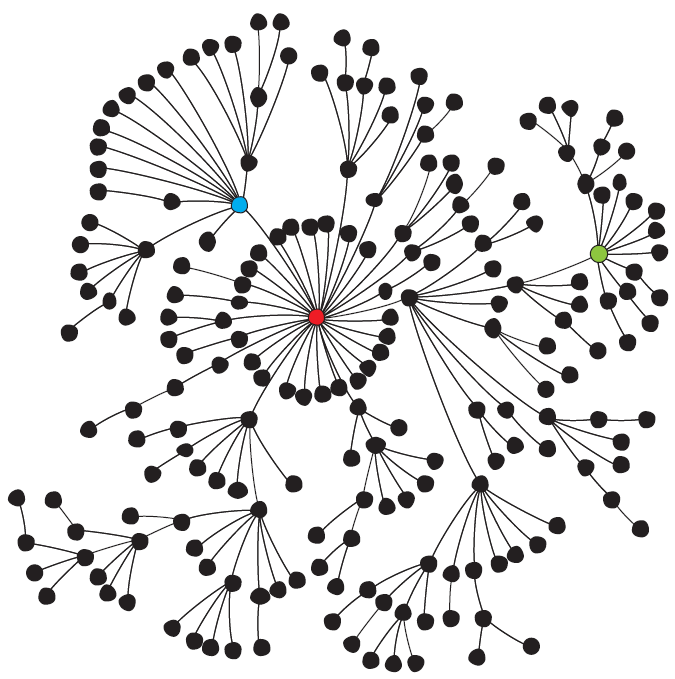
\includegraphics[width=0.4\textwidth]{images/scale-free-network.png}};

    \node (proc1) at (-3.5,2) [draw,thick,minimum width=2cm,minimum height=1cm,rounded corners=10pt] {Process 1};
    \node (proc2) at (-3.5,-2) [draw,thick,minimum width=2cm,minimum height=1cm,rounded corners=10pt] {Process $n$};

    \node (file1) at (0,2) [draw,thick,minimum width=2cm,minimum height=1cm,rounded corners=10pt] {GCV list 1};
    \node (file2) at (0,-2) [draw,thick,minimum width=2cm,minimum height=1cm,rounded corners=10pt] {GCV list $n$};
    
    \node (file_final) at (3,0) [draw,thick,minimum width=2cm,minimum height=1cm,rounded corners=10pt] {Final GCV list};
    
    \draw node[circle, minimum size=2cm, red, fill=red, fill opacity=0.2] (nodes1) at (-7.0,1.5)  {};
    \draw node[circle, minimum size=2cm, red, fill=green, fill opacity=0.2] (nodes2) at (-7.0,-1.5)  {};

    \draw[line width=2pt, loosely dotted] (-3.5,1) -- (-3.5,-1);
    \draw[line width=2pt, loosely dotted] (0,1) -- (0,-1);
    
%     \draw[red] (-12.0,9.5) rectangle (-1.0,9.0);
%     \draw[red] (-12.0,8.55) rectangle (-1.0,8.05);
    
    \draw[line,thick, ->] (nodes1) -- node[above] {chunk 1} (proc1) {};
    \draw[line,thick, ->] (nodes2) -- node[above] {chunk $n$} (proc2) {};
    \draw[line,thick, ->] (proc1) -- node[above] {GCVs} (file1) {};
    \draw[line,thick, ->] (proc2) -- node[above] {GCVs} (file2) {};
    \draw[line,thick, ->] (file1) -- (file_final.north west) {};
    \draw[line,thick, ->] (file2) -- (file_final.south west) {};

  \end{tikzpicture}
  \caption[Parallelisation process for the GCV computation]{Illustration of the parallelisation process for the GCV computation. For an input network, we split the nodes into different chunks and assign each chunk to a process. Each process computes the GCVs only for his chunk of nodes and writes them to an output file. At the end, all the GCV lists from the output files are assembled together into one final list. During the assembly process, the final GCV list is also sorted by node entry in order to easily visualise all the GCVs and to simplify our consistency checks.}
  \label{fig:parallelisation_process}
  \end{center}
\end{figure}%

%%%%%%%%%%%%%%%%%%%%%%%

\begin{figure}
\begin{lstlisting}
for each child process
{
  /* spawn a new process and store its PID */
  pids[proc_index] = fork();
  if (current process is a child)
  {
    /* open file suffixed by process number */
    FILE* out_file = fopen(out_name + proc_index, "w");
    /* find the nodes that the child needs to process */
    nodes_to_process = [CHUNK_SIZE * proc_index, CHUNK_SIZE * proc_index + 1]
    /* compute the GCV list and write them to the output */
    compute_gcv(input_graph, out_file, nodes_to_process);
    /* the child process closes the file and terminates */
    fclose(fp_out);
    return 0;
  }
}

/* Parent process waits on all children to finish execution */
for each child process
{
  waitpid(pids[proc_index]);
}
\end{lstlisting}
\caption[Pseudocode for the parallelisation logic]{Pseudocode for the parallelisation logic that is implemented in file \lstinline|e_gdv.cpp|. Note that the actual GCV computation takes place in the \lstinline|compute_gcv| function. The reason why the output file pointer is passed to this function is because we want each process to write the GCV signatures to the output files on the fly, as soon as they are computed. This helps us debug the software more easily and also avoid "out of memory" problems when processing large network files which have more than 11.000 nodes.}
\label{fig:pseudocode_parallelisation}
\end{figure}

Because of the way we chose to implement parallelisation, some processes tend to finish earlier than other. Even if every process computes the GCV for the same number of nodes in the network, computing the GCV for hub nodes takes considerably longer because they have large neighbouring subgraphs. As a result, some processes finish early while others get stuck with the GCV computation for some hub nodes. However, this limitation tends to become less obvious as the size of the input network increases. One way to overcome this problem is to redistribute the computation to the processes that finish early.

In order to evaluate the speedup from parallelisation, we repeatedly perform the GCV computation on the PPI, WTN and Metabolic networks using a variable number of processes and network size. Each experiment is also repeated 5 times and the average running time is reported. The machine we run the experiments is the \lstinline|Bionets02|, having the following specifications\footnote{The CPU type and memory size are taken from the output of the \lstinline|lshw| command. The specifications of the AMD Opteron 6282 SE processor are taken from the www.cpu-world.com website.}:
\begin{itemize}
 \item cpu: 4 x AMD Opteron(tm) Processor 6282 SE @ 2600MHz
 \begin{itemize}
  \item Number of cores: 16 
  \item Data width: 64 bit
  \item Level 1 cache size: 8 x 64 KB 2-way associative shared instruction caches, 16 x 16 KB 4-way associative data caches
  \item Level 2 cache size: 8 x 2 MB 16-way associative shared exclusive caches
 \end{itemize}
 \item memory: 125GB
\end{itemize}


We therefore calculate on \lstinline|Bionets02| the speedup obtained on the Human PPI, Human Metabolic and 2010 World Trade network as the number of processes increases from 1 to 64. The speedup $s_n$ when using $n$ processes is calculated as follows:
$$ s_n = 100\left(\frac{T_{1}}{T_{n}} - 1\right)$$\
where $T_{n}$ is the wall-clock time of execution when using $n$ processes, while $T_1$ is the wall-clock time of the serial execution. The final value is multiplied by 100 so that we can express it in percentage terms. Figure \ref{fig:time_threads} shows the speedup for the PPI, Metabolic and WTN networks. Each experiment has been run 5 times and the average running times $T_n$ have been used to compute the final speedup. When the number of processes is 2, we don't get any speedup in the execution, but as the number of processes increases, some speedup is clearly visible for the PPI and WTN networks. The Metabolic network only shows some speedup when 64 processes are running the computation. The PPI and the WTN networks also show a considerable speedup at the end, when executing the computation on 64 processes. It should be noted that the speedup of WTN becomes greater than the equivalent speedup of the PPI network when more than 32 processes are used.

\begin{figure}[H]
  \centering
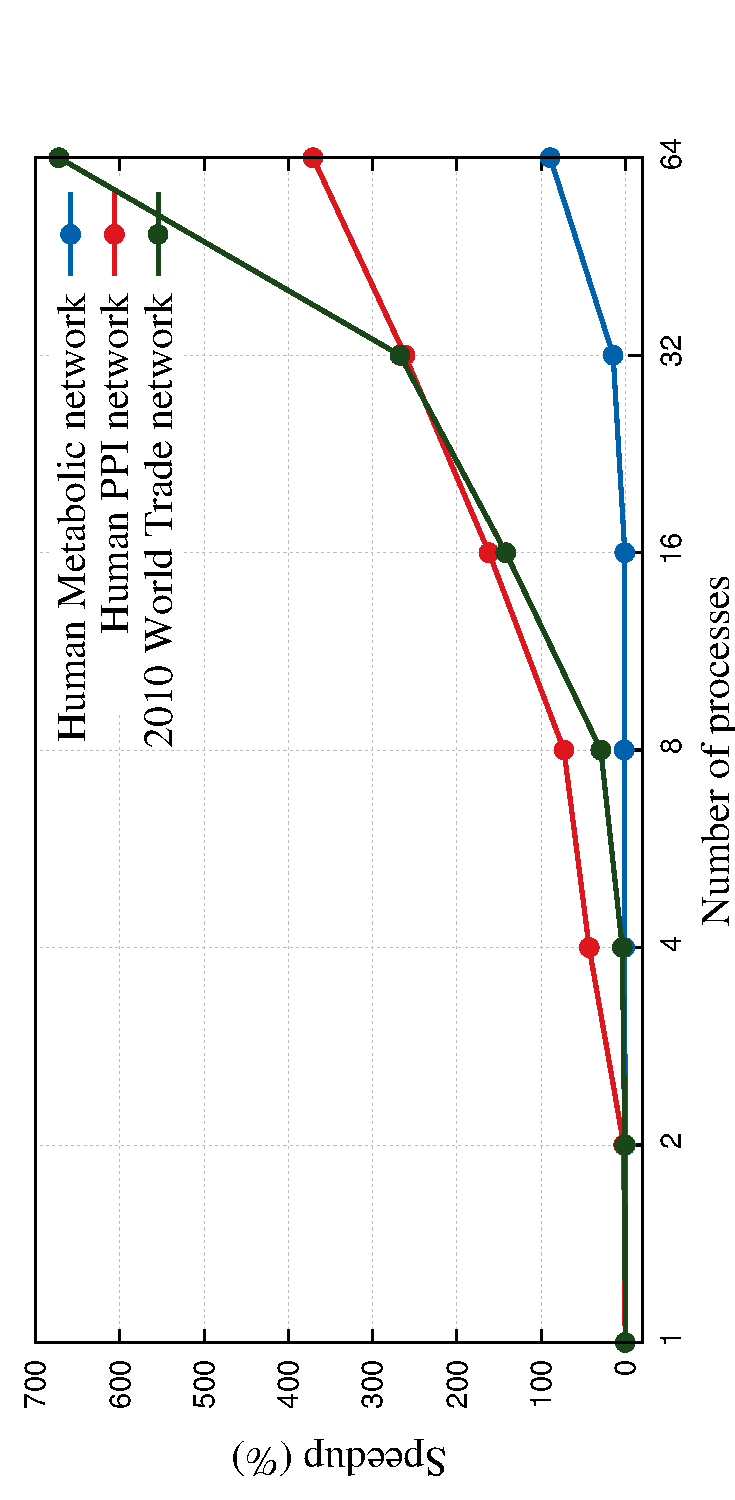
\includegraphics[angle=-90,scale=0.6]{../code/final_results/parallelisation_results/nr_processes2}
\caption[Parallelisation - speedup for PPI, Metabolic and 2010 WTN networks]{Speedup gained from parallelisation as the number of processes increases. The following three different networks have been tested: A human PPI network, a human metabolic network and a 2010 World Trade network (WTN). Although not immediately obvious from the graph because of the logarithmic $X$ axis, the speedup trend is linear in the number of processes. A maximum speedup of 680\% and 380\% is obtained for the WTN and the PPI network respectively when 64 processes are used.}
\label{fig:time_threads}
\end{figure}

After evaluating the speedup of the parallelisation, we are now interested to see how the execution time changes when we increase/decrease the problem size. In order to test for different problem sizes, we take a large network and randomly remove edges from it. We therefore generate networks that contain 50\%, 60\%, \dots , 100\% of the edges of the initial network. We then compute the execution time (wall-clock time) on each of these incomplete networks for a different number of processes. For each process and network size, 5 trials are run and the average execution time is reported. Figure \ref{fig:problem_size} shows the results obtained for this experiment. When the problem size is small, the execution time is fast regardless of the number of processes used. However, as the network size increases, the speedup gains from parallelisation become apparent, because the difference between lines widens. Eventually, when 64 processes are used, the execution time on the full network is approximately 32 seconds, 
which is 3-4 times faster than the equivalent execution time with 1 process. Note that the apparent inconsistencies between the PPI results in figure \ref{fig:time_threads} and the last column from figure \ref{fig:problem_size} might be because of the fact that the \lstinline|Bionets02| might have had other services from users running in the meantime that could have affected the performance.


\begin{figure}[H]
  \centering
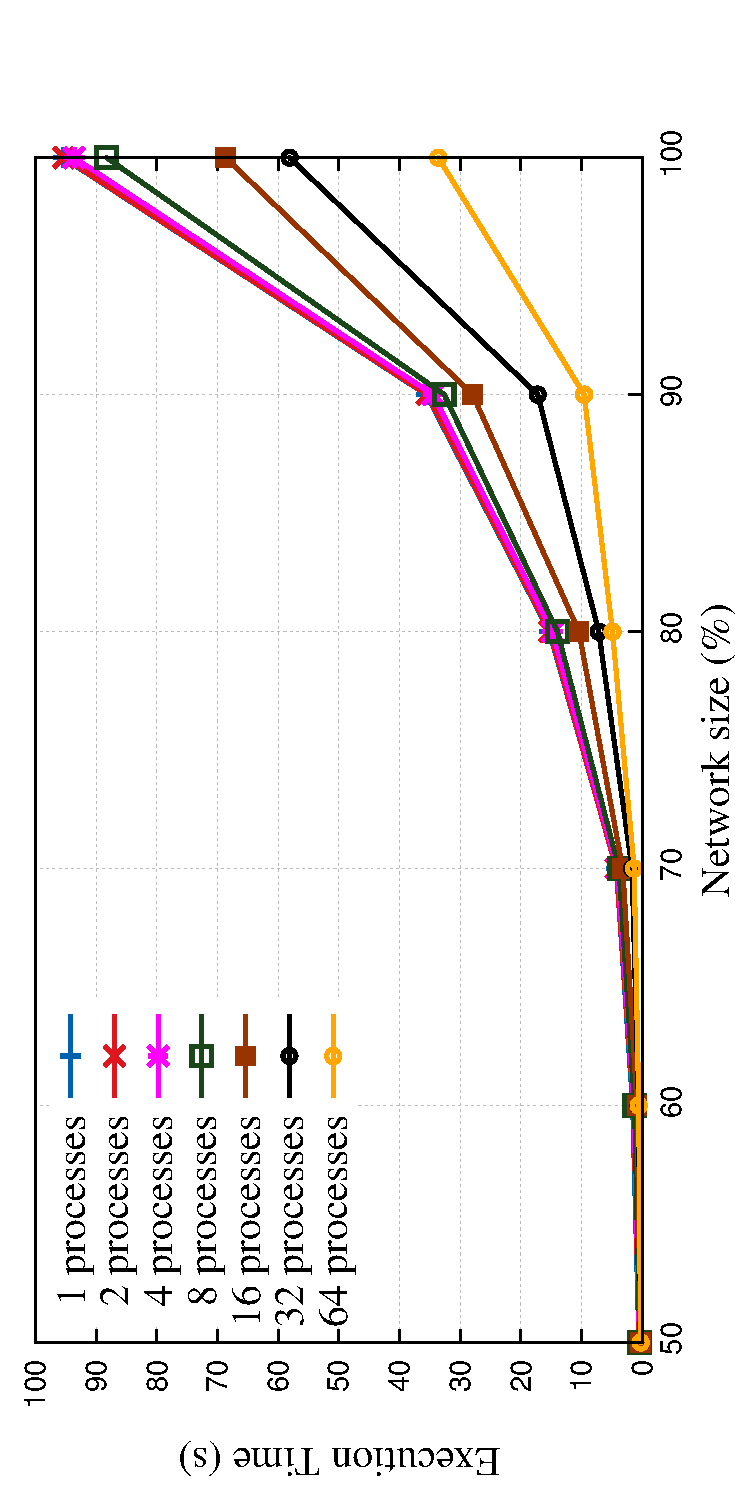
\includegraphics[angle=-90,scale=0.6]{../code/final_results/parallelisation_results/problem_size_human_ppi2}
\caption[Parallelisation - Execution time as the network size increases]{Execution time plotted for different number of processes as the network size increases. The input network used is the Human PPI network, and a network size of $p\%$ refers to the percentage of edges that were kept from the original network. For all network sizes, one can easily notice that the execution time gets faster as the number of processes increases. These results suggest that the gains in parallelisation are noticeable only for large networks.}
\label{fig:problem_size}
\end{figure}

The network that had the longest average runtime was the PPI network, with an execution time ranging from 95 seconds (1 process) to 32 seconds (64 processes). Although an execution time of 95 seconds is not problematic for our experiments, other PPI networks\footnote{the PPI networks from BioGRID - Full version, see section \ref{sec:cca_ppi_intro}} we have experimented with have taken around 10 hours to finish using 64 parallel processes. Moreover, other networks such as the literature network\footnote{We have also experimented with literature networks, which are networks of characters from a book. However, the results were not significant so we have not included them in this report.} of the Bible have taken several days to finish using 64 parallel processes. The reason the GCV computation takes so long to finish on these networks is because some processes get stuck with computing GCVs for hub nodes, which have very large neighbouring graphs.

In conclusion, parallelisation of GCV computation was a key part of the project that enabled us to run more experiments faster and to exploit all the computational resources of our machines. Some of the experiments on the PPI and literature networks would not have been possible without parallel computation.

\subsection{Pearsons's GCV correlation matrix}
\label{sec:metho_pears}

 In the background section \ref{pearsons_background}, we introduced the Pearson's GDV correlation matrix for a given graph. Similarly, the \emph{Pearson's GCV correlation matrix} can also be computed in order to find out which graphlets cluster together. This is important because graphlets that cluster together have a similar behaviour and also correlate with the same functional annotations. We present to the reader the steps used for computing the \emph{Pearson's GCV correlation matrix}, which uses the GCV (Graphlet Cluster Vector) instead of the GDV (Graphlet Degree Vector):
\begin{enumerate}
 \item We compute the Graphlet Cluster Vector (GCV) for every node in the
input network
 \item We then construct samples $ S_i, i\in {1,2,3, .. ,29} $
containing all the frequencies of the graphlet of type $i$ found in the GCVs of
the nodes. The length of $S_i$ would be equal to $N$, the number of nodes in the network.
 \item We compute the Pearson's correlation coefficient for each pair of samples $ (S_i, S_j) $ and we write them in the 29x29 correlation matrix $
C$ at position $(i,j)$.
\end{enumerate}

The program that computes the GCV correlation matrix has been written without using any library functions. Nevertheless, it took me a few of hours to identify some bugs and memory leaks. Using GDB and Valgrind has proven to be extremely helpful for this task. I also implemented my own function that computes the Pearson's coefficient for two samples $X$ and $Y$ and tested it using an excel spreadsheet that computed the correlation coefficient in parallel.

Unfortunately, the first heat maps that we get for the three main network classes (PPI, Metabolic and Trade) are not easy to interpret. See the initial image (top-left corner) from figure \ref{fig:heatmap_process}, which shows the original heat map obtained for the Human PPI network. Most of the graphlets display a high correlation (at least 0.5) and because of that we cannot distinguish clusters easily. Similar results are obtained for the other two networks: Human Metabolic and WTN. In order to identify which graphlets cluster together, we apply two main modifications to the matrices:
\begin{itemize}
 \item Normalisation: We normalise the correlation values so that they lie more evenly in the (0,1) range.
 \item Hierarchical clustering: In order to better identify clusters of graphlets that are highly correlated with each other, we perform hierarchical clustering on the set of 29 graphlet signatures.
\end{itemize}


\rowcolors{1}{blue1}{blue2}


%%%%%%%%%% GCV computation process %%%%%%%%%%%%%

\newcommand{\cellsizegcvtable}{1.45}

\newcommand{\gcvtable}{
\begin{tabular}{p{\cellsizegcvtable cm}p{\cellsizegcvtable cm}p{\cellsizegcvtable cm}p{\cellsizegcvtable cm}p{\cellsizegcvtable cm}p{0.5cm}}
 Graphlets    & GCV (node 1) & GCV (node 2) & GCV (node 3) & GCV (node 4) & \dots \\
 G1 & 2 & 3 & 6 & 9 & \dots \\ 
 G2 & 1 & 10 & 23 & 0 & \dots \\ 
 G3 & 0 & 3 & 5 & 14 & \dots \\ 
 G4 & 4 & 9 & 6 & 2 & \dots \\ 
 \dots &  \dots & \dots & \dots & \dots & \dots\\
 G29 & 1 & 14 & 6 & 0 & \dots \\  
\end{tabular}
}

\begin{figure}[h]
  \begin{center}
  \begin{tikzpicture}[scale=1.0,auto,swap,post/.style={->,shorten >=3pt,>=stealth',thick}]


    \node[inner sep=0pt] (1a) at (-9.0, 2.0) {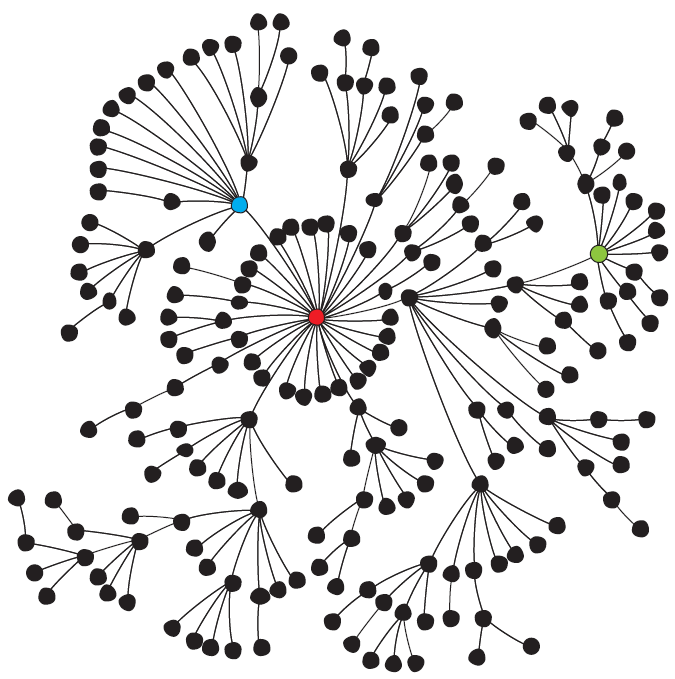
\includegraphics[width=0.4\textwidth]{images/scale-free-network.png}};
    \node[inner sep=0pt] (2a) at (-6.5, 9.0) {\gcvtable};
    \node[inner sep=0pt] (3a) at (-0.0, 2.0) {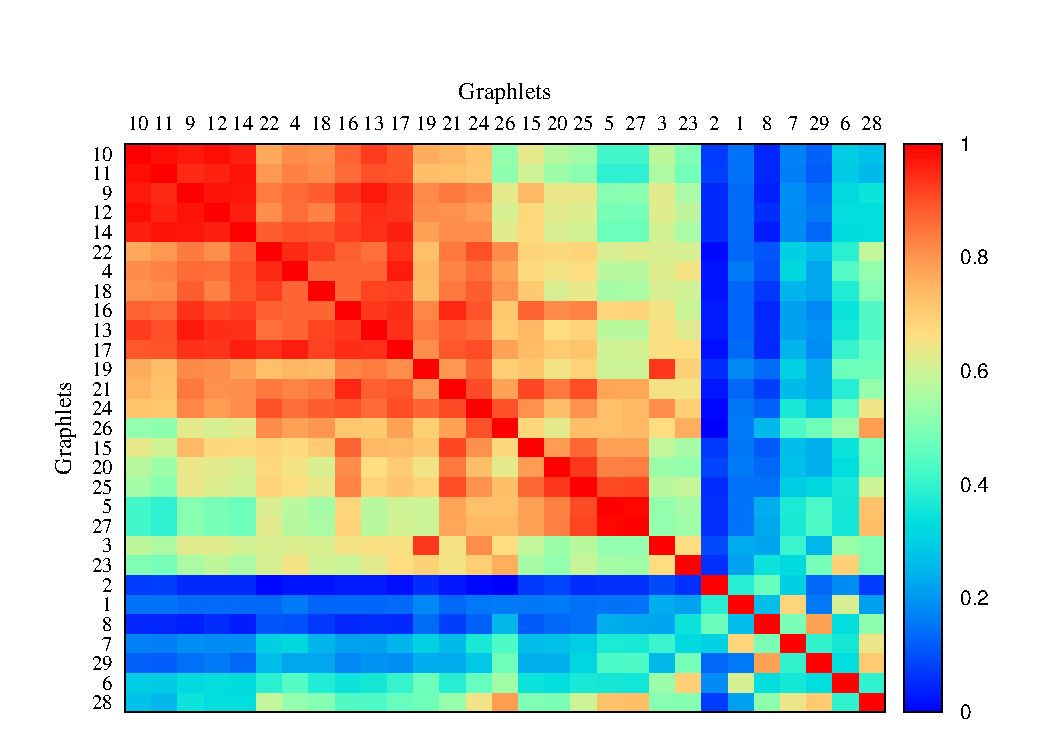
\includegraphics[scale=0.7]{../code/final_results_norm1/trade_2010_thresholded/heatmap_pearsons_hclust_trade_2010_thresholded2.pdf}};
    \node[text width=10em] (4a) at (2.5, 8.7) {$\rho(i,j) = $ Pearson's correlation between row vectors $i$ and $j$ };
    \node (5a) at (2.5, 1) {};
    \node (gcv_src) at (-1.0, 8.7) {};
    
    \draw[red] (-12.0,9.5) rectangle (-1.0,9.0);
    \draw[red] (-12.0,8.55) rectangle (-1.0,8.05);
	  
   \draw[post] (1a) -- node[right] {Graphlet Cluster Vectors (GCVs)} (1a |- 2a.south);
%     \path[hi, line width=1.0]  (4a)  -- (5a);
    \draw[post,rounded corners=5pt] (4a.south)-|(5a.north);
    \draw[post,rounded corners=5pt] (gcv_src) -- node[above] {} (gcv_src -| 4a.west) ;
    
  \end{tikzpicture}
  \caption[Computation process of the Pearson's GCV correlation matrix]{Computation process of the Pearson's GCV correlation matrix. For an input network, we compute a table of the GCV signatures for all the nodes in the input network. Afterwards, we compute the Pearson's correlation coefficient $\rho(i,j)$ between each pair of row vectors $i$ and $j$ and store it at position $M[i,j]$ in the correlation matrix $M$.}
  \label{fig:gcv_corr_process}
  \end{center}
\end{figure}%

%%%%%%%%%%%%%%%%%%%%%%%


% \begin{figure}[H]
%   \centering
%   \hbox{\hspace{-1cm}
%   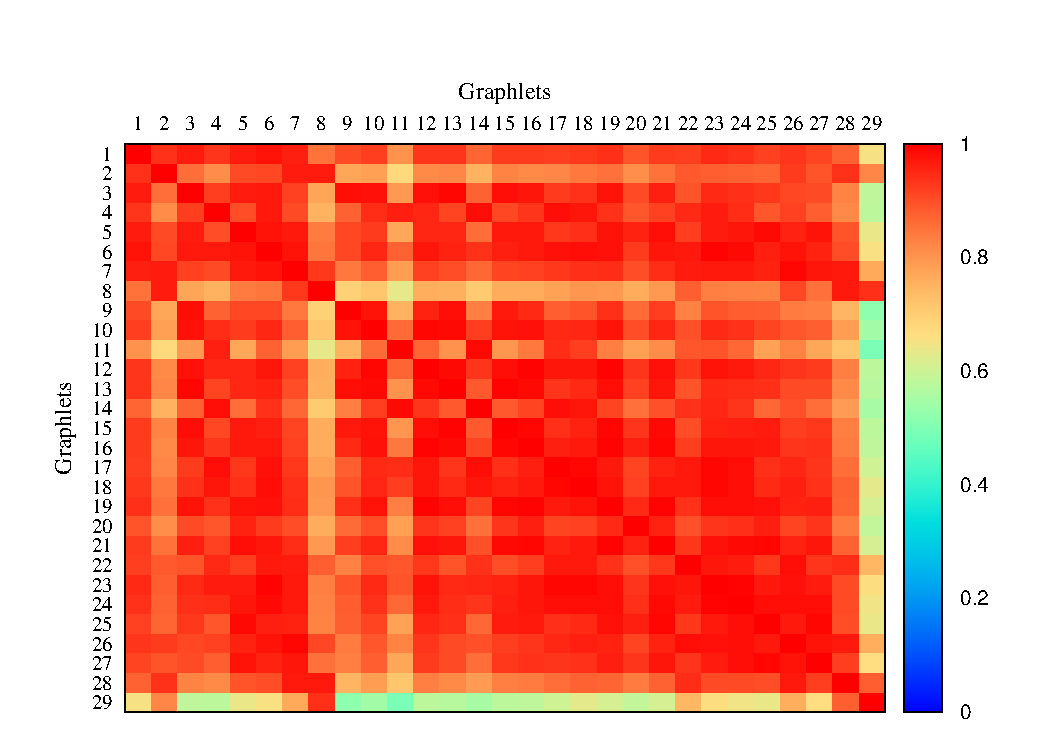
\includegraphics[scale=1.0]{../code/final_results/human_ppi/heatmap_pearsons_human_ppi2.pdf}}
%   \caption{Heatmap for the Pearson's GCV correlation matrix of the Human PPI network}
%   \label{ppi_heatmap}
% \end{figure}


\subsection{Normalisation}

Two main normalisation steps have been performed in order to spread out the correlation values over the (0,1) range:
\begin{enumerate}
 \item Feature scaling
 \item Polynomial scaling
\end{enumerate}

By feature scaling we denote a uniform scaling that makes the data fit on the (0,1) range. On the other hand, polynomial scaling applies a polynomial function to the input value. They are formally defined as follows:
\begin{mydef}
Let $X$ be a population and $min(X)$, $max(X)$ be the minimal respectively maximal value in $X$. Feature scaling is a transformation that converts each element $x \in X$ into an element $x'$ such that:
\begin{equation}
 x' = \frac{x - min(X)}{max(X) - min(X)}
\end{equation}
\end{mydef}


\begin{mydef}
Let $X$ be a population. Polynomial scaling is a transformation that converts each element $x \in X$ into an element $x'$ such that:
 $$x' = x^n$$ 
\end{mydef}



For each matrix, feature scaling is first applied followed by polynomial scaling. For both feature scaling and polynomial scaling, the set of all entries in the 2D matrix are used as the population vector $X$. After applying feature scaling, all the entries in the correlation matrix are converted to the (0,1) range. This results in both the input and output of the polynomial scaling to also be in the (0,1) range, regardless of the parameter $n$ that is used. 


\subsection{Hierarchical clustering}

Hierarchical clustering is a method that clusters data points according to how similar they are. In our case the data points were the 29 GCV correlation vectors, and the similarity measure used was given by the Euclidean distance. See section \ref{hier_clust} for background information on hierarchical clustering. The reason for clustering them is because we need to find out which graphlets are similar and which ones are different with each other. The graphlets that are similar probably have some common properties that we are able to identify and interpret.

We have used the python library \lstinline|Scipy| to run hierarchical clustering. We first calculate a distance matrix using the \lstinline|Scipy.spatial.distance|. This symmetric matrix stores the distances between every two data points as a 2D matrix. Afterwards, the hierarchical clustering is performed with the function call \lstinline|scipy.cluster.hierarchy.linkage(dist_matrix, method='complete')|. The method parameter refers to the type of hierarchical clustering that is performed. We have chosen to use Complete linkage\footnote{Complete linkage groups clusters together according to the shortest distance between the farthest points in the sets (see the definition for complete linkage in section \ref{hier_clust}).} because it avoids the so-called \emph{chaining phenomenon} of single linkage, where clusters are forced together due to outlier data points being close to each other, even though the majority of the data points might actually be away from each other. It has also been shown that complete 
linkage tends 
to create clusters of similar diameter \cite{everitt2001hierarchical}.

Each Pearson's correlation matrix is first normalised using both feature scaling and polynomial functions and then hierarchically clustered. We shall refer to this process as the \emph{Pearson's GCV correlation matrix life cycle}. More details about its implementation aspects can be found in section \ref{sec:life-cycle_framework}. Figure \ref{fig:heatmap_process} shows the \emph{Pearson's GCV correlation matrix life cycle} for the Human PPI network. One can clearly see that the initial matrix is very hard to interpret, having all correlations very high. On the other hand, the final matrix is very easy to interpret and clearly shows graphlet clusters formed along the diagonal. In this example, we used a a $4^{th}$ degree polynomial, but for other networks we found that other polynomial functions offer better results. Chapter \ref{chp:applications} presents the key results of the Pearson's matrices applied to different network classes.

%%%%%%%%%% Heatmap life cycle %%%%%%%%%%%%%

% Define the arm and angle options
\def\myarm{1cm}
\def\myangle{0}
\tikzset{
  arm/.default=1cm,
  arm/.code={\def\myarm{#1}}, % store value in \myarm
  angle/.default=0,
  angle/.code={\def\myangle{#1}} % store value in \myangle
}

% Define the myncbar to path
\tikzset{
    myncbar/.style = {to path={
        % We need to calculate a couple of coordinates to help us draw
        % the path. 
        let
            % Same as (\tikztotarget)++(\myangle:\myarm)
            \p1=($(\tikztotarget)+(\myangle:\myarm)$)
        in
            -- ++(\myangle:\myarm) coordinate (tmp)
            % Find the projection of the (tmp) coordinate
            % on the line from the target to p1
            --  node[below] {\hspace{1.0em}\begin{tabular}{c} $4^{th}$ degree polynomial scaling: \\ $x' = x^4$ \end{tabular}} ($(\tikztotarget)!(tmp)!(\p1)$)
            -- (\tikztotarget)\tikztonodes
    }}
}


\begin{figure}[h!]
  \rowcolors{1}{}{}
  \hspace{-3.0em}
  \begin{tikzpicture}[scale=1.0,auto,swap,post/.style={->,shorten >=3pt,>=stealth',thick}]

    \node[inner sep=0pt] (orig) at (0.0, 8.0) {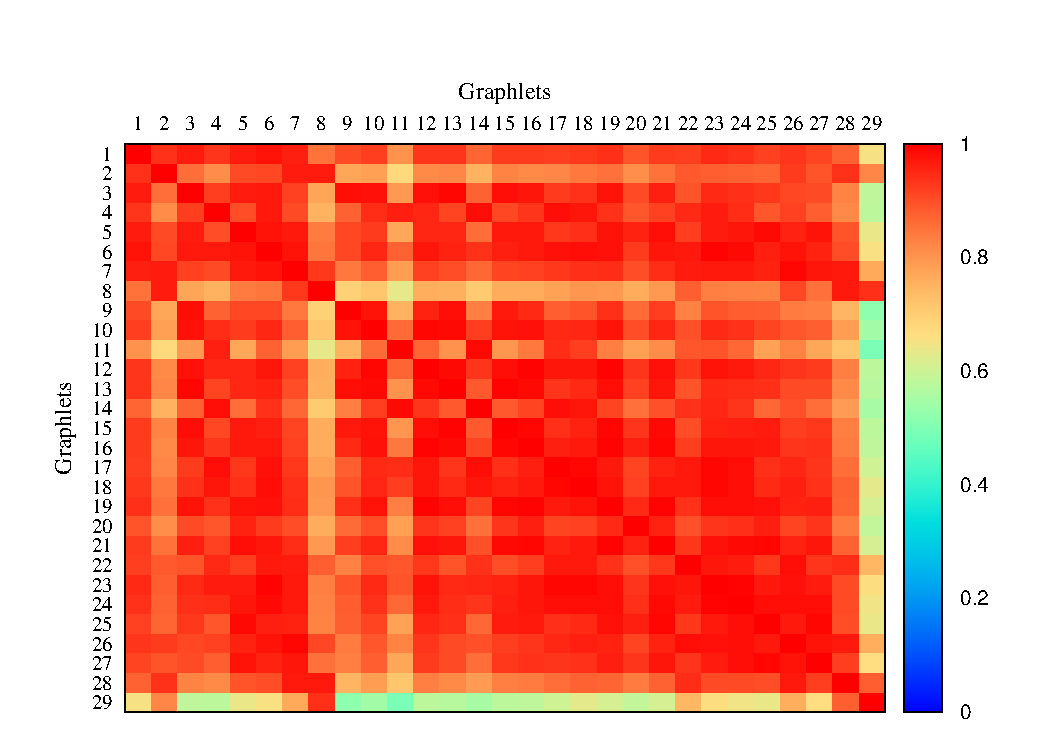
\includegraphics[scale=0.5]{../code/final_results/human_ppi/heatmap_pearsons_human_ppi2.pdf}};
    \node at (orig.north) {\textbf{Initial matrix}};
    \node[inner sep=0pt] (feature_scaled) at (0.0, 0.0) {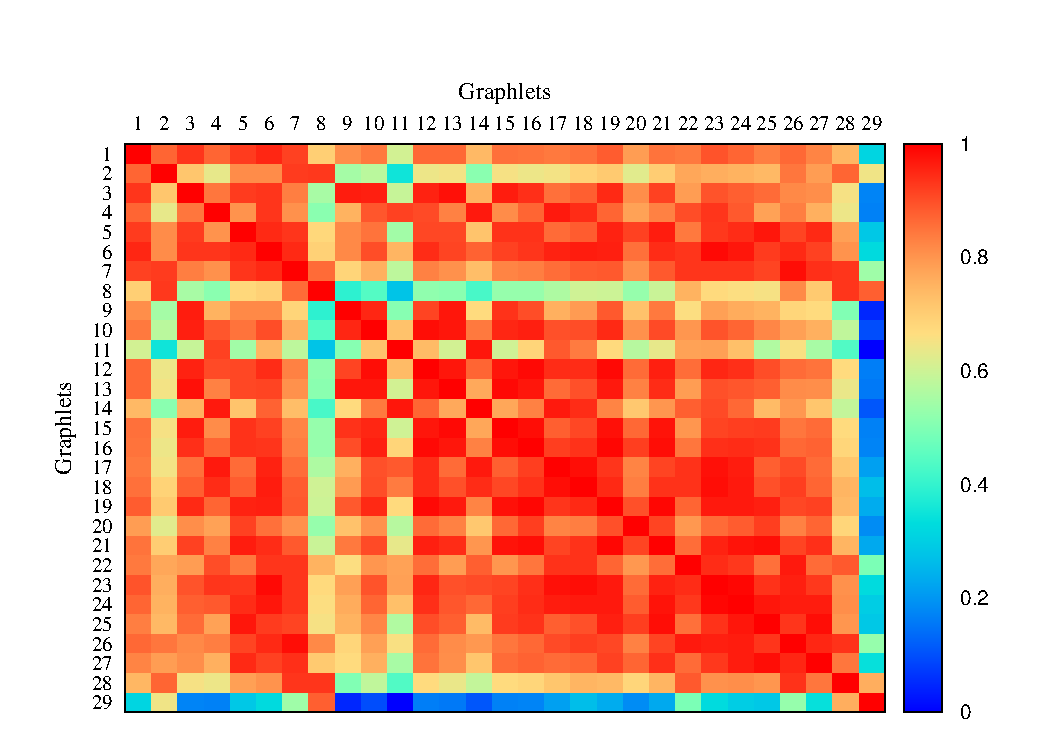
\includegraphics[scale=0.5]{../code/final_results/human_ppi/heatmap_pearsons_normalized_human_ppi2.pdf}};
    \node[inner sep=0pt] (poly4) at (9.0, 0.0) {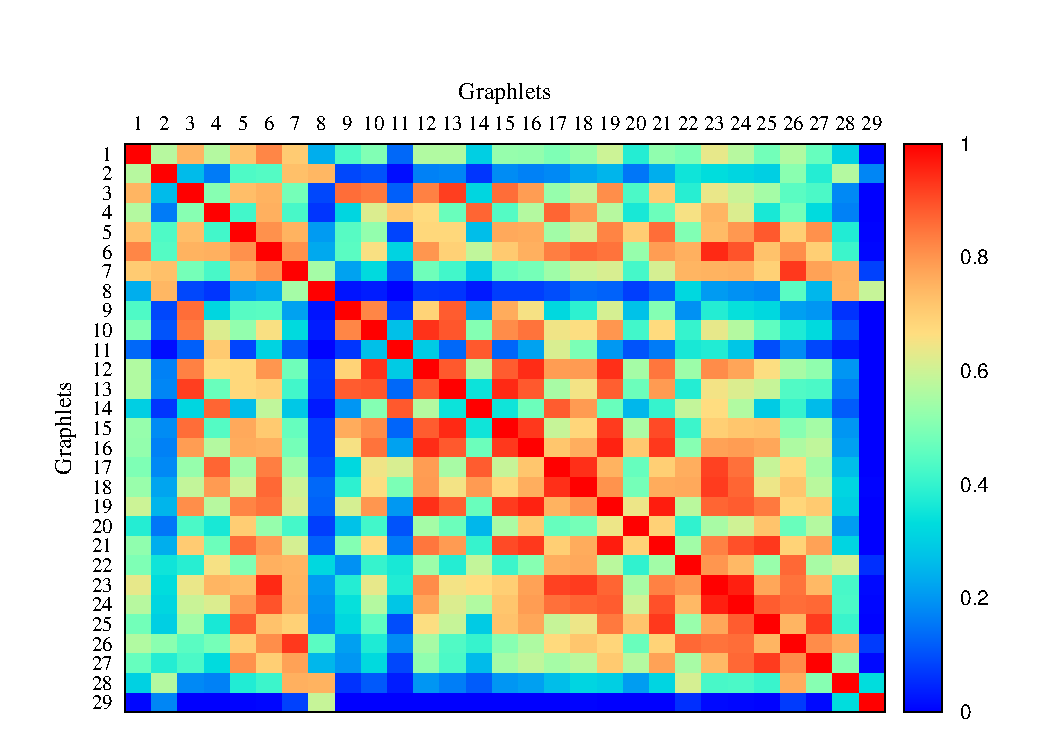
\includegraphics[scale=0.5]{../code/final_results/human_ppi/heatmap_pearsons_normalized_human_ppi-poly-42.pdf}};
    \node[inner sep=0pt] (hclust) at (9.0, 8.0) {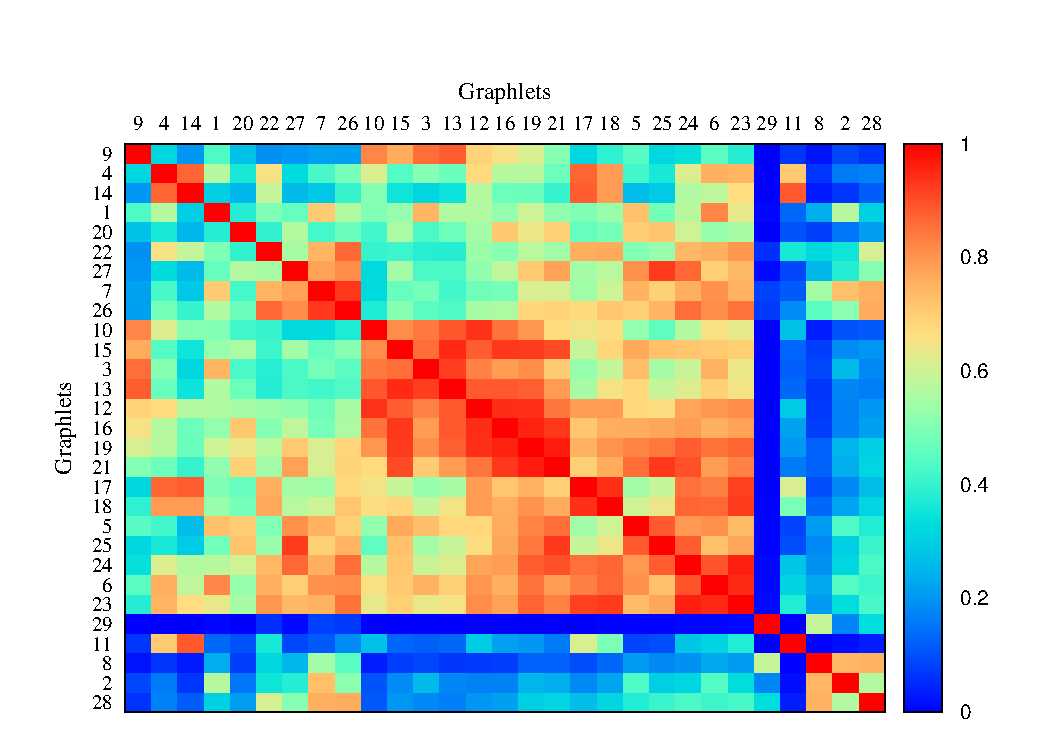
\includegraphics[scale=0.5]{../code/final_results/human_ppi/heatmap_pearsons_hclust_human_ppi-poly-42.pdf}};
    \node at (hclust.north) {\textbf{Final matrix}};
    
    \draw[line,thick, ->] (orig) -- node[right] {\begin{tabular}{l} feature scaling: \\ $x' = \frac{x - min}{max - min}$ \end{tabular}} (feature_scaled) {};
    \draw [->,thick] (feature_scaled.south)  to[myncbar,arm=-0.5cm,angle=90]  (poly4.south);
    \draw[line,thick, ->] (poly4) -- node[right] {\begin{tabular}{l}hierarchical clustering\\(complete linkage)\end{tabular}} (hclust) {};


  \end{tikzpicture}
  \caption[Pearson's GCV correlation matrix life cycle for the Human PPI network]{Pearson's GCV correlation matrix life cycle for the Human PPI network. The initial Pearson's GCV correlation matrix is on the top-left corner and the final matrix is on the top-right corner, after feature scaling, polynomial scaling and hierarchical clustering operations are applied. One can see that in the final matrix graphlet clusters are distinguished more easily compared to the initial matrix. The operation order is anti-clockwise. When feature scaling, the range of the correlations $[min, max]$ is scaled to $[0,1]$. After performing polynomial scaling using a $4^{th}$ degree function, the correlations are lowered even more. Finally, after applying hierarchical clustering, similar graphlets cluster together along the diagonal. Hierarchical clustering uses complete linkage for grouping GCVs and the Euclidean distance to compute the difference between GCVs.}
  \label{fig:heatmap_process}
\end{figure}%

%%%%%%%%%%%%%%%%%%%%%%%

\subsection{Canonical Correlation Analysis}

Graphlets only give us information about the topology of the network connections. However, in order to associate them with node functions or annotations, we need to correlate the GCV with a vector of node annotations. Canonical Correlation Analysis (CCA) is able to do exactly this and also give us a p-value, that can quantify the significance of the result. The theory behind CCA is given in background section \ref{cca_background}. In this section, we present how we applied CCA in our experiments and discuss implementation details.

% Discuss about Darren's scripts, how I modified them
Initially, I experimented with CCA using three different implementations:
\begin{itemize}
 \item \lstinline|Python Scikit|: a Python implementation that is based on algorithms by Jacob A. Wegelin \cite{wegelin2000survey}. The problem with this implementation is the poor documentation available.
 \item \lstinline|Matlab|: based on two books by Krzanowski, W. J. \cite{krzanowski2000principles} and Seber, G. A \cite{seber2009multivariate}. The documentation is good, but the implementation does not provide canonical cross-loadings.
 \item Darren Davis's \lstinline|R| script: Darren Davis is a collaborator of N. Pr\v{z}ulj who has previously applied CCA on GDV signatures. His \lstinline|R| implementation also performs some preprocessing of the data points and covariance matrices, such as scaling, centring\footnote{The data points are centred around the origin} and regularisation\footnote{If the covariance matrix is singular, a weighted identity matrix is added to it. More formally, if the covariance matrix of the data points is $S$, then $S' = S + \lambda I$}. This implementation is also accompanied by some python scripts that can preprocess all the trade networks for a given range of years.
\end{itemize}

We have decided to use Darren Davis's script, mainly because it is able to calculate cross-loadings and it also had 5 accompanying python scripts that preprocess the economic networks. Therefore, we refactored the \lstinline|R| script in order to allow several parameters to be passed from the command line. On the other hand, the preprocessing python scripts have been extensively modified to deal with the new GCV signature and for enabling them to process different annotation files, such as EC numbers (see section \ref{metabolic_annotations}) or Boone's and von Mering's annotations (see section \ref{ppi_annotations}).

\hilight{Discuss about how I converted the annotation files}

% Add reference with example pictures and tables once they have been added.

Darren Davis's \lstinline|R| script gives us all the canonical correlation eigenvectors, with their associated correlation and p-values and writes them to a text file. The eigenvectors are sorted in descending order by their correlation strength, so the first eigenvector is the most significant. We therefore created a parser for this file that finds the first eigenvector and produces a \LaTeX\ table with all the cross-loadings and the respective overall correlation and p-value. This script has been used for generating all the CCA tables in this report. We have also created another script that creates a vector graphics image containing the following:
\begin{itemize}
 \item an indicator list on the left-hand side where is element is coloured from green (1) to red (-1) according to their canonical cross-loading.
 \item a top-right panel containing the graphlets with the highest canonical cross-loading.
 \item a bottom-right panel containing the graphlets with the lowest canonical cross-loading.
 \item a gradient bar in the middle measuring correlation where the graphlets and indicators are connected.
\end{itemize}

This script is written in Python and generates fragments of \lstinline|Tikz| code that can be used by \LaTeX to generate the image. In order to get the images in their final state, further manual modifications are performed. The images are very intuitive to understand and will be used extensively during the presentation. They are also included in this report in figures \ref{fig:all_trade_cca_unnorm_black}, \ref{fig:all_trade_cca_black} and \ref{fig:ppi_cca_black}. However, we don't include them for all CCA results in the report because they don't give the exact correlations which are required for a careful analysis.

\subsection{Network life cycle framework}
\label{sec:life-cycle_framework}
In order to be able to run all our experiments in an automatic fashion and for a variety of networks, we implemented a few \emph{network life cycle frameworks} that take a network and run all the statistical experiments automatically. The frameworks are defined by commands in a Makefile that chain a variety of scripts. We wrote two main classes of such frameworks: 
\begin{enumerate}
 \item Pearson's GCV Correlation matrix life cycle: used for computing all the correlation matrices and generating several types of heat maps.
 \item Canonical Correlation life cycle: used for preprocessing a network and its annotation file and applying CCA on them.
\end{enumerate}

Both of these are described in more detail in the following subsections.

\subsubsection{Pearson's GCV correlation matrix life cycle}

The \emph{Pearson's GCV correlation matrix life cycle} takes an input network and computes several GCV correlation matrices and their corresponding heat maps. Several environment variables need to be set in order to run it, such as the network source folder, network file, generated folder\footnote{The generated folder is used for storing all the program results} and the GCV normalisation type\footnote{A binary value that decides whether the GCV is normalised or not.}. The steps that are performed in the life cycle are as follows:
\begin{enumerate}
 \item Initial file handling: Several directories are created and input files are copied over.
 \item GCV computation using \lstinline|e_gdv.cpp|\footnote{The name of the script is derived from "extended gdv", because at the time we started writing the script we were not decided on the name for the new signature.}
 \item Average network GCV computation
 \item Computation of the Pearson's GCV correlation matrix
 \item Computation of 4 types of normalised correlation matrices\footnote{The matrices are normalised with first, second, third and fourth degree polynomials. The higher the degree, the stronger the contrast between correlation values will become.}
 \item Hierarchical clustering on all the correlation matrices
 \item Heat map generation of all the correlation matrices using \lstinline|gnuplot|
\end{enumerate}


\subsubsection{Canonical Correlation Analysis life cycle}

A different framework was set up for Canonical Correlation Analysis. In order to run CCA on an input network, several preprocessing steps are required that transform the GCV and annotation files. For the World Trade network, the steps performed by the CCA life cycle are defined below:
\begin{enumerate}
 \item Initial file handling: the output folders are created and input files are copied over.
 \item Conversion of the GCV dump file to a CSV file for each of the 48 networks over the period 1962-2010.
 \item Aggregation of the above per-year GCV CSV files into a single GCV file.
 \item Aggregation of the economic indicator files into a single CSV file. Country/year entries with incomplete data are dropped.
 \item Augmentation of the basic economic indicators with composed economic indicators (e.g. GDP per capita x Population to get the total GDP of a country).
 \item Alignment of the GCV entries with the final economic indicators.
 \item execution of the actual Canonical Correlation Analysis
\end{enumerate}

\hilight{add the python files for each of these steps. the listing env has some probs with wrapping though}

The CCA life cycle described above is specific for the Trade networks. Similar frameworks were created for the other networks, which use different types of annotations. The steps performed are similar, but they use different parameters and one different preprocessing script that converts the indicators to a CSV file. It must be noted that the Python scripts performing the above steps are based on scripts created by Darren Davis for the GDV-based CCA.

\subsection{Unit testing}

Throughout the project we implemented a small suite of unit tests that checks the basic functionality of the GCV signature computation. We used the \lstinline|BOOST| unit testing framework written in \verb!C++! because of the following reasons:
\begin{itemize}
 \item The core algorithm that computes the GCV signature has also been written in \verb!C++!, which made integration easy.
 \item The \lstinline|BOOST| testing framework has very useful features such as:
 \begin{itemize}
  \item Grouping test cases into suites.
  \item The ability of running multiple, independent tests in parallel.
  \item The possibility of seeing the progress of long and complex tests.
 \end{itemize}
 \item There exists a variety of online tutorials and learning materials on the \lstinline|BOOST| testing framework
\end{itemize}

We wrote unit tests that check for the correctness of the GCV signature on PPI, Metabolic and World Trade networks. Moreover, we also tested the GCV on a small number of toy networks and compared the results with GCV signatures that were calculated by hand. Furthermore, we also tested the parallel computation in the following manner:
\begin{enumerate}
 \item For a given input network, we compute the GCV signature list several times, using an increasing number of processes.
 \item We compare each of the generated GCV lists for consistency. 
\end{enumerate}

This parallelisation test actually helped us discover a bug in the code caused by a null pointer exception, which only occured when 2 or more processes were used. This only affected a few of the processes that accessed the illegal area of the virtual memory and stopped their execution. As a result, the resulting GCV dump was incomplete, and this aspect was not immediately obvious without a close examination of the GCV list. 

The unit tests in our suite can be run using the Makefile command: \lstinline|make test|. This will execute all the tests in the test suite. One can also run individual tests or a subset of all the tests in the suite. Running two tests on the WTN network using 16 and 32 processes for the GCV computation produces an output similar to the one in figure \ref{fig:unit_test_output}.

\definecolor{test_green}{HTML}{003300} % 
\definecolor{test_blue}{HTML}{0033CC} % 

\lstdefinestyle{base}{
  language=C,
  emptylines=1,
  breaklines=true,
  basicstyle=\ttfamily\color{black},
  moredelim=**[is][\color{test_green}\textbf{}]{@}{@},
}

\begin{figure}[H]
\begin{lstlisting}[style=base,escapechar=!]
!\textcolor{test_blue}{Running 2 test cases...}!

!\textcolor{test_blue}{Running:}! ./e_gdv trade_2010_thresholded.gw test_bank/trade_2010_thresholded 16
Finished parsing the LEDA file
Waiting on the children ...Children have finished processing. Assembling the files...Running: cat test_bank/trade_2010_thresholded.0* > test_bank/trade_2010_thresholded.ndump2;rm test_bank/trade_2010_thresholded.0*

@Test successful@

!\textcolor{test_blue}{Running:}! ./e_gdv trade_2010_thresholded.gw test_bank/trade_2010_thresholded 32
Finished parsing the LEDA file
Waiting on the children ...Children have finished processing. Assembling the files...Running: cat test_bank/trade_2010_thresholded.0* > test_bank/trade_2010_thresholded.ndump2;rm test_bank/trade_2010_thresholded.0*
% 
@Test successful@


@*** No errors detected@

\end{lstlisting}
\caption[Command-line output when running two unit tests on the 2010 World Trade network]{Command-line output when running two unit tests on the 2010 World Trade network using 16 and 32 processes. For each test, the input network LEDA file is first parsed and then the parent waits until all children finish their processing. When the children processes finish their work, their output files are assembled together and checked for consistency.}
\label{fig:unit_test_output}
\end{figure}
